\documentclass[11pt,a4paper]{article}
\usepackage{theme/lmuthesis}
\usepackage{svg}
\usepackage{algorithm2e}
\usepackage{multicol}
\DontPrintSemicolon
\usepackage[acronym]{glossaries}

\graphicspath{images/}

\newacronym{aabb}{AABB}{Axis-aligned Bounding Box}
\newacronym{obb}{OBB}{Oriented Bounding Box}
\newacronym{bvh}{BVH}{Bounding Volume Hierarchy}
\newacronym{lbvh}{LBVH}{Linear Bounding Volume Hierarchy}
\newacronym{sah}{SAH}{Surface Area Heuristic}
\newacronym{rdh}{RDH}{Ray Distribution Heuristic}
\newacronym{phr}{PHR}{Progressive Hierarchical Refinement}
\newacronym{simd}{SIMD}{Single Instruction, Multiple Data}
\makeglossaries

% this for draft water mark
\setboolean{release}{true}

\ifthenelse{\boolean{release}}{
}{
    \usepackage{draftwatermark}
    \SetWatermarkText{DRAFT}
    \SetWatermarkScale{1}
}

% meta informations
\department{Institut f\"ur Informatik}
\lfe{Lehr- und Forschungseinheit Medieninformatik}
\professor{Prof.\ Dr.\ Butz}
\type{Bachelor's Thesis}
\title{Progressive BVH Refinement in Interactive Ray Tracing}
\author{Christian Schmidt}
\email{nichtchristianschmidt@gmail.com}
% TODO: Fill out END
\bearbeitungszeitraum{06.05.2021 bis 23.09.2021}
\supervisor{Changkun Ou}
\taskdescription{
    % TODO: Format description
    \begin{description}
        \item[Progressive BVH Refinement in Interactive Ray Tracing]
        \item[Problem Statement] 
        Path tracing in real time become avaliable on the GPU side in recent years due to the recent advances in image denoising techniques, such as NVIDIA DLSS.

        It is interesting to optimize and render everything directly on the CPU in real time for reasonably smaller scenes.
        \item[Tasks]
        \begin{itemize}
            \item Implement a multi-threaded CPU ray tracer
            \item Profile and identify the bottleneck of your ray tracer implementation
            \item Benchmark and compare the performance difference between your CPU ray tracer and an equivalent CUDA ray tracer
            \item Summarize your findings in a thesis and presenting them to audiences
        \end{itemize}
        \item[Requirements]
        \begin{itemize}
            \item Have experience or projects using C++ (or Go)
            \item General knowledge about computer graphics
        \end{itemize}
    \end{description}
}
\acknoledgement{
    The meshes used to evaluate the path tracer are courtesy of Morgan McGuire's Computer Graphics Archive\cite{McGuire2017Data} and the Standford 3D Scanning Repository. 
    I would like to thank my advisor Chankun Ou for his patience and for all his feedback and input in countless meetings. 
    His contributions in the form of the bench\cite{ou20bench} framework and a Bayesian optimizer\cite{ou19bo} helped my work significantly.
    Finally, I would like to thank my CPU for taking quite the beating in several benchmarking and rendering sessions. 
}
\abstract{
    Path tracing is a rendering technique that simulates how light travels through a scene, producing physically correct images, albeit at a significant computational cost. Only in recent years has this technology become viable in real-time rendering through powerful denoising techniques and special purpose hardware. This thesis continues this work by first presenting a self-contained overview over the basics of path tracing. A closer look at CPU based interactive path tracing is provided and its performance is evaluated based on a path tracer written from scratch in Go. A particular focus is set on acceleration data structures, which are used to optimize the ray tracing process significantly. Consequently, the state-of-the-art bounding volume hierarchy construction algorithm called progressive hierarchical refinement is presented and applied to the interactive application. Finally, a novel approach for evaluating the build-trace trade-off of that algorithm is proposed and the optimization problem is solved using grid search and Bayesian optimization.
    \\
    \\
    \\
    \\
    \\
    \\
    \\
    \\
    Path Tracing ist eine Technik zur Bildsynthese, welche den Lichttransport durch eine Szene simuliert. Dadurch werden physikalisch plausible Bilder erzeugt, wenn auch auf Kosten eines hohen Rechenaufwands. Erst in den letzten Jahren wurde diese Technologie auch im Real-Time Rendering realisierbar, vor allem durch leistungsstarke Rauschunterdr{\"u}ckungsverfahren und spezielle Hardware. Diese Arbeit kn{\"u}pft an diese Fortschritte an, indem zun{\"a}chst ein in sich geschlossener {\"U}berblick {\"u}ber die Grundlagen des Path Tracing pr{\"a}sentiert wird. Anschlie{\ss}end wird CPU basiertes interaktives Path Tracing n{\"a}her betrachtet und dessen Leistung basierend auf einem in Go von Grund auf neu geschriebenen Path Tracer evaluiert. Ein besonderer Fokus liegt auf Datenstrukturen, die der Beschleunigung des Ray Tracing Prozesses dienen. Im Zuge dessen wird der Algorithmus "Progressive Hierarchical Refinement", welcher zur Konstruktion von Bounding Volume Hierarchien dient und dem neusten Stand der Technik entspricht, vorgestellt und in die interaktive Applikation integriert. Zuletzt wird ein neuer Ansatz zur Evaluierung des Konstruktion-Render-Ausgleichs des Algorithmus vorgeschlagen und das Optimierungsproblem durch Rastersuche und Bayessche Optimierung gel{\"o}st.
}

\notation{
    Here the notation used throughout this thesis is described. Vectors are denoted by bold lowercase letters, e.g. \textbf{v} and matricies by bold upper case letters, e.g. \textbf{M}. Scalars are lowercase, italicized letters, e.g. $c$. Points are uppercase, e.g. $P$. The components of a vector are accessed as 
    \[
        \textbf{v}  = \left[ \begin{array}{r}v_x\\v_y\\v_z\end{array} \right]
                    = \left[ \begin{array}{r}v_0\\v_1\\v_2\end{array} \right]
                    = \left[ \begin{array}{rrr}v_x&v_y&v_z\end{array} \right]^\top
    \]
    where the latter shows the vector transposed, i.e. a column becomes a row. The dot product between to vectors is written as $a\cdot b$. \\\\A matrix \textbf{M} can be written in the following ways:
    \[
        \textbf{M}  = \left[ \begin{array}{rrr}
                            m_{00} & m_{01} & m_{02}\\
                            m_{10} & m_{11} & m_{12}\\
                            m_{20} & m_{21} & m_{22}
                        \end{array} \right]
                    = \left[ \begin{array}{rrr} \textbf{m}_0 & \textbf{m}_1 & \textbf{m}_2\end{array} \right]
    \]
    where \textbf{m}$_i, i\in\{0,1,2\}$, are the column vectors of the matrix.
    
}

\begin{document}
\makecover
\maketaskdescription
\makededication
\makeabstract
\makenotation
\maketoc
% optional:
% \listoffigures
% \listoftables
\cleardoublepage
\section{Introduction}
Ray tracing is foremost a rendering technique simulating how light travels through a scene and thus inherently producing very realistic images. Effects that need to be simulated explicitly in the contrasting approach of rasterization, such as shadows, reflections and refractions are achieved by default, albeit introducing a substantial computational cost. It is this simplicity paired with the high quality output, that made the method a staple in offline rendering where the relatively long rendering time can be tolerated. In real-time settings where the time to render single frames is limited, ray tracing is a rather poor fit and requires a number of optimizations to push its performance to a sufficient point. Only in recent years has that point been reached and surpassed far enough to open the technology up for a consumer market, especially by utilizing special-purpose hardware. A particularly noteworthy milestone in that regard is NVIDIA's Turing architecture\cite{nvidia2017turing}, which is built in a way that accelerates basic ray tracing operations while also facilitating other software technologies essential to the process, most importantly more advanced denoising techniques. However, the availability of such graphic cards is still limited, so software based solutions remain an interesting topic which this thesis tries to tackle. 

% TODO: Add references to the corresponding sections 
In particular, this thesis provides a self-contained overview over the basics of real-time ray tracing as well as some implementation details of an interactive CPU path tracer written from scratch, which might be useful as a starting point for further research and more optimizations. Furthermore, a closer look at bounding volume hierarchies is presented, and the approach of progressive hierarchical refinement\cite{hendrich_parallel_2017} is introduced as a state-of-the-art algorithm to construct such acceleration structures. The integration of the aforementioned approach into an interactive path tracer is described and validated, as this was still an open question. Finally, two methods for optimizing hyperparameters related to the construction algorithm in real-time are introduced, evaluated and discussed.
\section{Preliminaries}
This section introduces all basic concepts needed to follow along with the rest of this thesis, while also putting some focus on notable historical work. Additional topics that are not part of the thesis, but still important to the overall context, are also touched on. To keep this work self-sustained, everything is explained from the ground up, no previous knowledge required.
\subsection{Path Tracing}
% TODO: Citation style, only cite year and write name
At the core of any ray tracing approach is the concept of a ray, usually in three-dimensional space. In this work the following representation is used.
\[P(t)=O+td\]
% TODO: Introduce math notation
Where the origin $O$ is some point within the scene space and the direction $d$ is some vector along which the ray travels in a straight line. Points along this line can be described using the distance $t$, with $P(0)=O$ and $P(1)=O+d$. 
% TODO: Add Ray tracing Figure
As illustrated in figure 1, this concept can be used to construct images. Rays are cast into a scene, originating at some common eye point and intersecting each pixel in the image plane to find its corresponding color. The first ray casting algorithm using such a technique was proposed by Appel\cite{appel1968}, only considering primary intersections and shadow rays towards a light source to determine whether a point is illuminated or not. Whitted\cite{whitted_improved_1980} expanded on that approach by introducing an algorithm that, upon finding an object intersection, generates secondary rays influencing the final pixel color. In addition to the previously mentioned shadows, these secondary rays allow rendering of reflections and refractions by recursively casting new rays in the reflection direction and blending all results. 
% TODO: Is it really more common?
A more common approach, especially in film and visual effects\cite{keller2015path_tracing_revolution}, is a closely related concept called path tracing\cite{kajiya_rendering_1986}. Instead of evaluating a single ray per pixel, multiple samples with slight offsets and random scattering are used to more accurately simulate light transport through a scene and approximate the rendering equation also introduced by Kajiya. Path tracing is a global illumination solution and thus produces more realistic results, while also allowing accurate rendering of distribution effects\cite{cook_distributed_1984} and inherently solving the problem of aliasing. 
\subsection{Path Tracing Optimizations}
The issue with path tracing is, that it requires many samples to produce plausible results as images without sufficient samples suffer from high-frequency noise. Tracing such a number of rays, while also maintaining interactive frame rates, simply is not possible at the moment and probably will not be in the foreseeable future, especially with Moore's law converging to an end. As a result, real-time path tracing would not be possible without optimizations reducing the rendering time by several orders of magnitudes. 
\subsubsection{Denoising}
A big leap towards reducing that number was achieved in recent years through the introduction of more advanced denoising techniques. Through denoising, the required samples-per-pixel can be reduced to a significantly lower number, going down to single sample with some techniques. Schied et al.~\cite{schied_spatiotemporal_2017} combines path tracing output with previous frame data and a noise free G-buffer generated using a rasterization pass, to feed a wavelet filter and produce a denoised, temporally stable sequence of images using only one path-per-pixel. Chaitanya et al.~\cite{chaitanya_interactive_2017} applies machine learning to the problem by using a convolutional neural network to map noisy input images to noise-free output. Other real-time reconstruction filters\cite{mara17towards,koskela2019bmfr} achieve similar results and opened up the door for real-time path tracing in the first place. However, denoising was not the focus of my work and will not be mentioned in the remainder of this thesis. Subsequently, the described path tracer produces noisy one sample-per-pixel output leaving the choice of denoising technique open, even though applying any denoising technique would be an interesting task for some future work.
% TODO: Metion DLSS?
% TODO: Add paragraph about importance sampling?
\subsubsection{Acceleration Data Structures}
Another essential optimization technique, and also the focus of this thesis, is improving path tracing itself by using acceleration data structures. As established, the essential operation in path tracing is finding intersections between a given ray and the traced scene. A naive approach would be to test the ray against all scene primitive, which in practice might be several million operations and thus too expensive. In practice, primitives are arranged in hierarchical data structures, so that only a reduced number of ray intersection calculations is necessary. Approaches for generating such data structures can be divided into two categories, space subdivision and object subdivision~\cite{macDonald1988space}.

The former works by splitting the scene space recursively into smaller subregions, building a rooted tree with references to the objects in its leaves. These trees might be binary, as first proposed by Fuchs et al.~cite{fuchs1980bsp}, or have a higher branching factor, often referred to as a KD-tree. While KD-trees generally have a lower depth, binary trees allow for simpler traversal, as only a two-way decision is needed at each step. 

Glassner\cite{glassner_space_1984} described one of the earliest approaches for generating octrees that, for each recursive step, splits the given subspace at the spatial median along all three axis, resulting in eight new subregions. Kaplan\cite{kaplan_use_1985} expanded on that idea by introducing a very similar implementation utilizing binary trees instead of octrees. Fujimoto et al.~\cite{fujimoto_arts_1986}, while also using octrees, achieved a significant speed improvement by using incremental integer arithmetic to optimize the traversal algorithm. Traversal is also what these approaches excel in. Space is divided into disjoint subregions which can be tested in the order a ray passes through them. If a hit is found, the traversal algorithm can be terminated without checking further tree nodes, which is not as trivial in object subdivision approaches. One of the limitation of such approaches is, that an object might be in multiple subregions at once, so multiple leaves might contain pointers to the same object. This is problematic, because an intersection with the given object that lies outside the associated subregion might be found and thus needs to be checked during the traversal step. A valid approach for clipping objects to solve this problem was described by Havran and Bittner~\cite{Havran02onimproving} together with other traversal improvements utilizing a new termination criteria. More modern KD-tree construction algorithms~\cite{roccia2012kdtree,choi2010sahKdTree,wu2011sahKdTree} make use of the Surface Area Heuristic (SAH)~\cite{MacDonald2005HeuristicsFR} further improving their performance.

While space subdivision approaches have previously been regarded as the best acceleration data structure~\cite{havrand2000comparison}, object subdivision has since caught up and overtaken~\cite{vinkler2015comparison}, making it the most popular approach for path tracing. In addition, bounding volume hierarchies are very beneficial in dynamic scenes~\cite{wald_ray_2007}, as they can be re-fit efficiently on scene changes. Because of these advantages, only object subdivision approaches will be considered in the following sections of this thesis. 

Object subdivision, mostly in the form a bounding volume hierarchy (BVH), was first mentioned by Clark~\cite{clark1976bvh} and also referenced by Whitted\cite{whitted_improved_1980} in his essential ray tracing paper. In contrast to space subdivision approaches, BVHs 
\section{Related Work}
\subsection{Denoising}
\label{denoising}
Efficient denoising techniques are essential to real-time path tracing, as only a limited number of samples-per-pixel is available for any given frame. While offline methods achieve the best quality, only interactive and real-time approaches are relevant in the context of this thesis. Yan et al.\cite{yan14denoising} proposed a sheared filtering approach that achieves interactive frame rates. Schied et al.\cite{schied_spatiotemporal_2017} proposed an approach that combines path tracing output and previous frame data with a noise free G-buffer generated using a rasterization pass to feed a wavelet filter. Mara et al.\cite{mara17towards} independently proposed a similar ray-tracing/rasterization hybrid method. They used a bilateral filter variant to achieve similar results. Chaitanya et al.\cite{chaitanya_interactive_2017} showed that neural networks can be used for denoising at interactive frame rates by using a convolutional neural network (CNN) to map noisy input images to noise-free output. In this approach, temporal noise was addressed by using recurrent connections in each layer of the CNN. Regression-based noise filtering produces higher quality output at the cost of more expensive computation. Koskela et al.\cite{koskela2019bmfr} were the first to implement a regression-based reconstruction pipeline that runs in real time. 

State-of-the-art denoising approaches are able to produce a denoised, temporally stable sequences of images using only one sample-per-pixel. However, denoising was not the focus of this work and will not be mentioned in the remainder of this thesis. Consequently, the implemented path tracer produces noisy one sample-per-pixel output leaving the choice of denoising technique open, even though applying any denoising technique would be an interesting topic for some future work.
\subsection{Space Subdivision}
Fuchs et al.\cite{fuchs1980bsp} proposed one of the first binary space partitioning trees, also referred to as kd-trees, which is built by recursively splitting the space along a given axis. This cut position is selected in a way that both sides contain a relatively equal number of objects. Glassner\cite{glassner_space_1984} described an approach for generating octrees that, for each recursive step, splits the given subspace at the spatial median along all three axis, resulting in eight new subregions. While trees with higher branching factors generally have a lower depth, binary trees allow for simpler traversal, as only a two-way decision is needed at each step. Kaplan\cite{kaplan_use_1985} expanded on Glassners idea by introducing a very similar implementation utilizing binary trees instead of octrees. Fujimoto et al.\cite{fujimoto_arts_1986}, while also using octrees, achieved a significant speed improvement by using incremental integer arithmetic to optimize the traversal algorithm. Havran and Bittner~\cite{Havran02onimproving} introduced additional traversal improvements utilizing a new termination criteria and a novel approach for clipping primitives. More modern kd-tree construction algorithms\cite{roccia2012kdtree,choi2010sahKdTree,wu2011sahKdTree} make use of the Surface Area Heuristic (SAH)\cite{goldsmith_automatic_1987,macdonald_heuristics_1990} further improving their performance. Li et al.\cite{li17parallelKD} proposed a construction algorithm based on Morton codes\cite{morton66curve} to enable a maximum level of parallelism. Hunt et al.\cite{hunt07lazybuild} proposed kd-tree construction from a given hierarchy. A similar approach for BVH construction is presented in section \ref{phr}
\subsection{Object Subdivision}
Bounding volume hierarchies were first mentioned by James Clark~\cite{clark1976bvh} and also referenced by Turner Whitted\cite{whitted_improved_1980}. Meister et al.\cite{meister21survey} published a report that reviews state-of-the-art BVH methods and discusses best practices. 

In the context of interactive and real-time rendering, construction speed is very crucial, especially when dealing with dynamic scenes. However, parallelizing the construction process is not straightforward. One parallel solution is a BVH based on Morton codes, which reduces the construction process to sorting primitives along the Morton curve\cite{morton66curve}. Sorting Morton codes with fixed length has a complexity of $O(n)$ and can be parallelized fairly efficiently. Such an approach was first proposed by Lauterbach et al.\cite{lauterbach09lbvh} as a top down GPU-based algorithm called \acrfull{lbvh}. A similar CPU based approach is elaborated further in section \ref{aux}. Pantaleoni and Luebke\cite{pantaleoni10hlbvh} proposed hierarchical LBVH, which combines LBVH with sweeping SAH in the upper levels of the tree and Garanzha et al.\cite{garanzha11hlbvh} applied binning SAH using Morton code prefixes as bin indices. Karras\cite{karras12lbvh} improved LBVH by using a special node layout and bottom-up reduction to construct the whole tree in parallel. Apetrei\cite{apetrei14lbvh} further improved the approach by constructing the tree and computing bounding boxes in one go, which was previously done in two seperate steps. Chitalu et al.\cite{chitalu20lbvh} combined LBVH with an ostensibly-implicit layout, which is the fastest construction algorithm to date\cite{meister21survey}.
Another improvement was presented by Vinkler et al.\cite{vinkler17morton} where Morton codes also encode the size of scene primitives. Hou et al.\cite{hou11bvh} proposed another GPU-base parallel algorithm for constructing kd-trees and BVHs by using partial breadth-first search and dumping results to CPU memory in between iterations to control GPU memory. 

While space subdivision approaches have previously been regarded as the best acceleration data structure~\cite{havrand2000comparison}, object subdivision has since caught up and overtaken~\cite{vinkler2015comparison}, making it the most popular approach for path tracing. Some of the advantages of bounding volume hierarchies include a predictable memory footprint, robust and efficient query and scalable construction. In addition, bounding volume hierarchies are very beneficial in dynamic scenes\cite{wald_ray_2007}, as they can be re-fit efficiently on scene changes. Because of these advantages, only object subdivision approaches will be considered in the following sections of this thesis.
\cleardoublepage
\section{Path Tracer}
\label{path_tracer}
This section presents a closer look at the general path tracing process and highlights key implementation details of the evaluated CPU path tracer.
\subsection{Pipeline}
\begin{figure}[H]
    \centering
    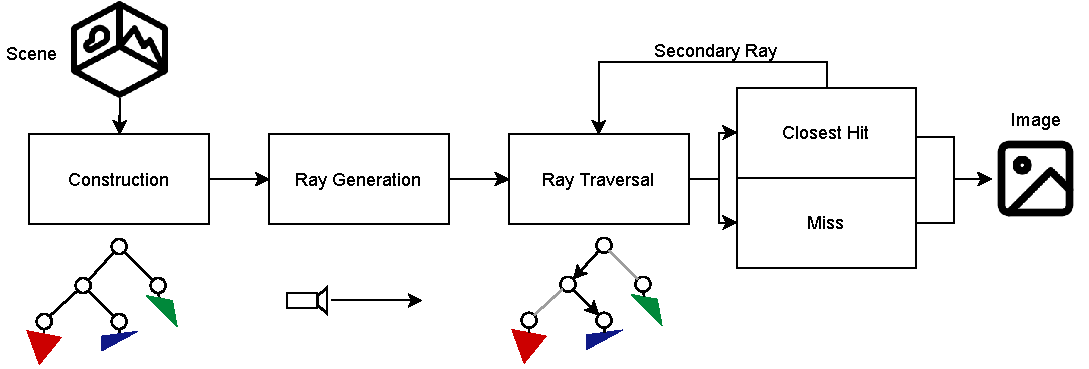
\includegraphics[width=400pt]{images/ray_trcing_pipeline.pdf}
    \caption{Visualization of path tracing process as a pipeline.}
    \label{fig:ray_pipeline}
\end{figure}
The graphics rendering process if often organized into a graphics pipeline\cite{sugerman09gramps}, so I generalized the path tracing process in a similar fashion (figure \ref{fig:ray_pipeline}). In the first stage of that pipeline the acceleration structure is created, which will be discussed further in section \ref{phr}. Given a static scene, this acceleration structure can be reused for multiple frames. Dynamic scenes require additional care though, as the acceleration structure either needs to be refit or rebuild on scene changes. The implemented uses a hybrid approach further elaborated in section \ref{phr_in_interactive}. The next stages are responsible for ray traversal and intersection testing. First, primary rays are generated from the camera's origin towards each pixel. Then, each ray has to traverse the acceleration structure to find the closest hit. Depending on whether or not this intersection has been found, either the closest hit shader, or the miss shader is called. Each shader can contribute to the color of the pixel, but only the closest hit shader spawns secondary rays. Note that my implementation uses implicit light sources instead of explicitly casting shadow rays. Secondary rays are fed back to the ray traversal stage and after reaching the maximum depth, the closest hit shader exits without creating any additional rays. The steps in these stages are embarrassingly parallel, however, because every ray is independent of the others, \acrshort{simd} instructions cannot be utilized. Consequently, each pixel is processed concurrently using multithreading.
\subsection{Intersection Tests}
A ray can be expressed using the parametric form 
\begin{equation} \label{eq:1}
    R(t)=O+t\textbf{d}
\end{equation}
where point $O$ defines the origin of the ray and vector \textbf{d} defines the direction along which the ray travels in a straight line. The path tracer supports two types of primitives, spheres and triangles. 
\subsubsection{Sphere}
Spheres are commonly used in ray tracing because of their simple and efficient intersection algorithm\cite{haines2019}. Given a sphere with center $C$ and radius $r$, all points $P$ at the surface of the sphere can be described by the equation:
\begin{equation} \label{eq:2}
    (P-G)\cdot(P-G)=r^2
\end{equation}
By substituting point $P$ in equation \ref{eq:2} by the equation of a ray (equation \ref{eq:1}) the intersection points between sphere and ray can be calculated. Simplifying the resulting equation leads to 
\[
    (\textbf{d}\cdot\textbf{d})t^2+2(\textbf{f}\cdot\textbf{d})t+\textbf{f}\cdot\textbf{f}-r^2 = at^2+b^t+c = 0
\]
which is a quadratic function. Consequently, it can be solved using 
\[
    t_{0,1}=\frac{-b\pm\sqrt{b^2-4ac}}{2a}
\]
with discriminant $\Delta=b^2-4ac$.
\begin{figure}[H]
    \centering
    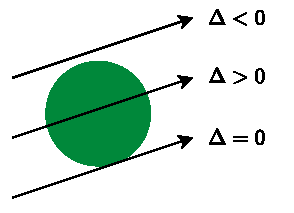
\includegraphics[width=150pt]{images/ray_sphere_intersection.pdf}
    \caption{Ray-sphere intersection test showing all three cases for discriminant $\Delta$.}
    \label{fig:sphere_intersec}
\end{figure}
As seen in figure \ref{fig:sphere_intersec}, if $\Delta<0$, the ray misses the sphere. If $\Delta=0$ the ray touches the sphere in one point and otherwise there are two values for $t$ that correspond to different intersection points. Inserting these $t$-values into equation \ref{eq:1} allows the calculation of intersection points $P_{0,1} = R(t_{1,2}) = O+t_{0,1}$\textbf{d}. The normal $n$ at a given intersection point is simply the vector from the spheres center $C$ to the intersection point $P$, i.e the normalized normal is calculated using $n=||P-C||$.

\subsubsection{Triangle}
Triangles have a long tradition in computer graphics, mainly because most geometry can be represented, or at least approximated, using them. Additionally, with 3 vertecies they can never be non-planar. While many ray-triangle intersection algorithms exist, the M{\"o}ller-Trumbore algorithm\cite{moeller97triangle} is still considered to be relatively fast and is often used as a comparison for other algorithms. Consequently, it is also used in this thesis. 

Using barycentric coordinates, a point $P$ on a triangle can be parameterized and expressed through two scalar values:
\[
    P(u,v) = (1-u-v)V_0 + uV_1 + vV_2
\]
where $V_0$, $V_1$ and $V_2$ are the vertices of given triangle and $(u,v)$ are the barycentric coordinates with $u\geq0$,  $v\geq0$ and $u+v\leq1$. Barycentric coordinates do not change when the triangle is transformed, which the M{\"o}ller-Trumbore algorithm exploits. Geometrically speaking, the algorithm translates the triangle to the origin and transforms it into a unit triangle in $y$ and $z$, with the ray direction aligned with $x$. This can be expressed as a system of linear equations:
\[
    \left[ \begin{array}{rrr}-\textbf{d}&(V_1-V_0)&(V_2-V_0)\end{array} \right]
    \left[ \begin{array}{r}t\\u\\v\end{array} \right] = O - V_0
\]
\begin{figure}[H]
    \centering
    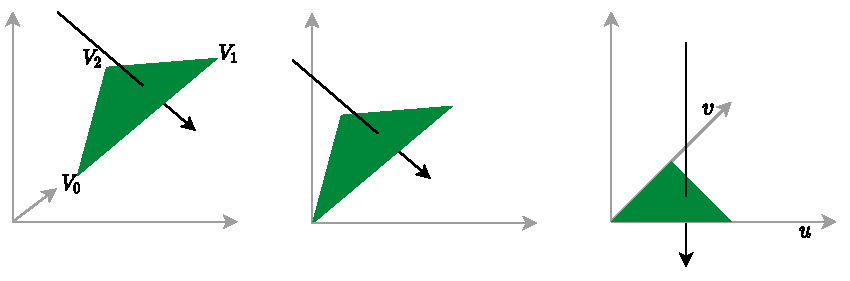
\includegraphics[width=400pt]{images/ray_triangle_intersec.pdf}
    \caption{Geometric representation of the transformations utilized in the M{\"o}ller-Trumbore algorithm.}
    \label{fig:triangle_intersec}
\end{figure}
Using Cramer's rule\cite{brunetti14cramersRule}, this system can be solved to obtain the distance $t$ from ray origin to intersection point and the corresponding barycentric coordinates $(u,v)$. Distance $t$ is again plugged into the ray equation to find the world coordinates of intersection point $P$ and the barycentric coordinates are used to interpolate the normal at $P$, given the vertex normals at $V_0$, $V_1$ and $V_2$.

\subsubsection{Axis-aligned bounding box}
Finally, bounding volume hierarchy traversal depends on a ray-bounding box intersection test. Axis-aligned bounding boxes are represented by the bounds $B^{min}$ and $B^{max}$, which define two planes for each dimension. The intersection distances $t$ between a given ray $R(t) = O+t\textbf{d}$ and a dimension $k$ can be computed fairly simple:
\[
    t^{min}_k = \frac{B_{k}^{min} - O_{k}}{\textbf{d}_{k}}
\]
\[
    t^{max}_k = \frac{B_{k}^{max} - O_{k}}{\textbf{d}_{k}}    
\]
Whether or not a ray intersects a box, can be determined by a few simple value comparisons, as seen in figure  \ref{fig:aabb_intersec}. The algorithm is optimized further by pre-computing sign and inverse direction for all rays and adding an early exit once it is clear the ray missed. 
\begin{figure}[H]
    \centering
    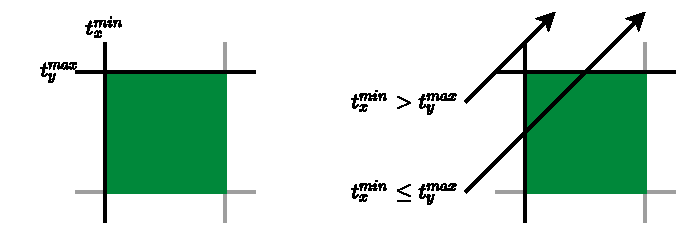
\includegraphics[width=400pt]{images/aabb_intersec.pdf}
    \caption{2D example of ray-AABB intersection. The top ray misses, while the bottom one hits the box.}
    \label{fig:aabb_intersec}
\end{figure}
\clearpage
\subsection{Materials}
Each primitive has an associated material. A material has an albedo specifying how reflective it is, i.e. how much color is contributed to the traced path, and an amount of emitted light. The scatter function differs between materials and is used to generate secondary rays. Note that it is also possible for materials to not scatter at all, which is used for light sources. 

Diffuse materials scatter rays in random directions. To achieve true Lambertian reflectance\cite{weik01lambert}, random points are picked on the surface of a unit sphere and added to the normal at intersection point. This results in a distribution of $cos(\Phi)$, where $\Phi$ is the angle from the normal. 

A smooth reflective material\cite{Greve2004ReflectionsAR} does not scatter rays in a random direction, so the resulting rays point purely in the reflection direction $\textbf{d}_r$ (figure \ref{fig:reflect_refract}):
\[
    \textbf{d}_r = \textbf{d} - 2\textbf{n}(\textbf{d}\cdot \textbf{n})
\]
where $\textbf{n}$ is the normalized normal at intersection point and $\textbf{d}$ is the direction of the incoming ray. For diffuse reflection a random vector is added to the reflected ray, similar to the above mentioned diffuse scattering.

Refractive materials\cite{Greve2004ReflectionsAR} utilize Snell's law to represent dielectrics like glass objects. Snell's law can be written as 
\[
    sin \theta' = \frac{\eta}{\eta'}sin \theta
\]
where $\theta$ and $\theta'$ are angles from the normal and $\eta$ and $\eta'$ are refractive indices. The refracted direction $\textbf{d}_t$, as shown in figure \ref{fig:reflect_refract}, can be split up into a parallel and a perpendicular part:
\[
    \textbf{d}_t=\textbf{d}_{\bot}+\textbf{d}_{\parallel}
\]
Solving for $\textbf{d}_{\parallel}'$ and $\textbf{d}_{\bot}'$ leads to:
\[
     \textbf{d}_{\bot}' = \frac{\eta}{\eta'}(\textbf{d}+(-\textbf{d}\cdot\textbf{n}) \textbf{n})
\]
\[
    \textbf{d}_{\parallel}' = - \sqrt{1-|\textbf{d}_{\bot}'|^{2}\textbf{n}}
\]
Adding both parts together, leads to the refracted direction $\textbf{d}_t$
\begin{figure}[H]
    \centering
    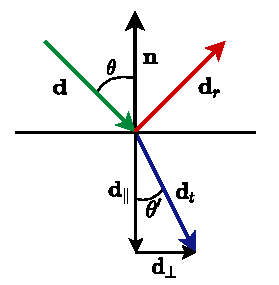
\includegraphics[width=200pt]{images/reflection_refraction.pdf}
    \caption{Figure showing how a ray's direction (green) is reflected (red) and refracted (blue).}
    \label{fig:reflect_refract}
\end{figure}
\subsection{Traversal}
\label{traversal}
To find the nearest intersection, bounding volume hierarchies are traversed in a top-down manner. Usually, this is done using a stack\cite{meister21survey} to store nodes that might contain an intersection. First, the root is pushed to the stack. While the stack is not empty, nodes are popped and checked for an intersection with their bounding box. In case the bounding volume is hit, either the nodes children are pushed onto the stack in the case of an interior node, or all primitives are tested when dealing with a leaf node. If no intersection with the bounding box is found or the distance to the intersection is bigger than previously found intersections, then the node can be discarded. Once the stack is empty, the closest intersection found is returned.

However, this method proved to be less efficient than using a recursive procedure as described in algorithm \ref{alg:traversal}. Given that the implementation is written for the CPU, this implicitly uses the CPU stack, which results in an equivalent execution as described above, albeit without explicitly managing a stack data structure.
\begin{algorithm}
\caption{Pseudocode of recursive BVH traversal}
\label{alg:traversal}
    \tcp{Start traversal at root}
    
    \SetKwFunction{FTraverse}{Traverse}
    \FTraverse{root}\;
    \;
    \SetKwProg{Fn}{Function}{:}{}
    \Fn{\FTraverse{node}}{
        \If{node.aabb not intersected} {
            \Return
        }
        \If{node is leaf} {
            \ForEach{primitive}{
                test for ray-primitive intersection
            }
        }
        \Else{
            \ForEach{child}{
                \FTraverse{child}
            }
        }
    }
\end{algorithm}
\cleardoublepage
\section{Progressive Hierarchical Refinement}
\label{phr}
\begin{figure}[H]
    \centering
    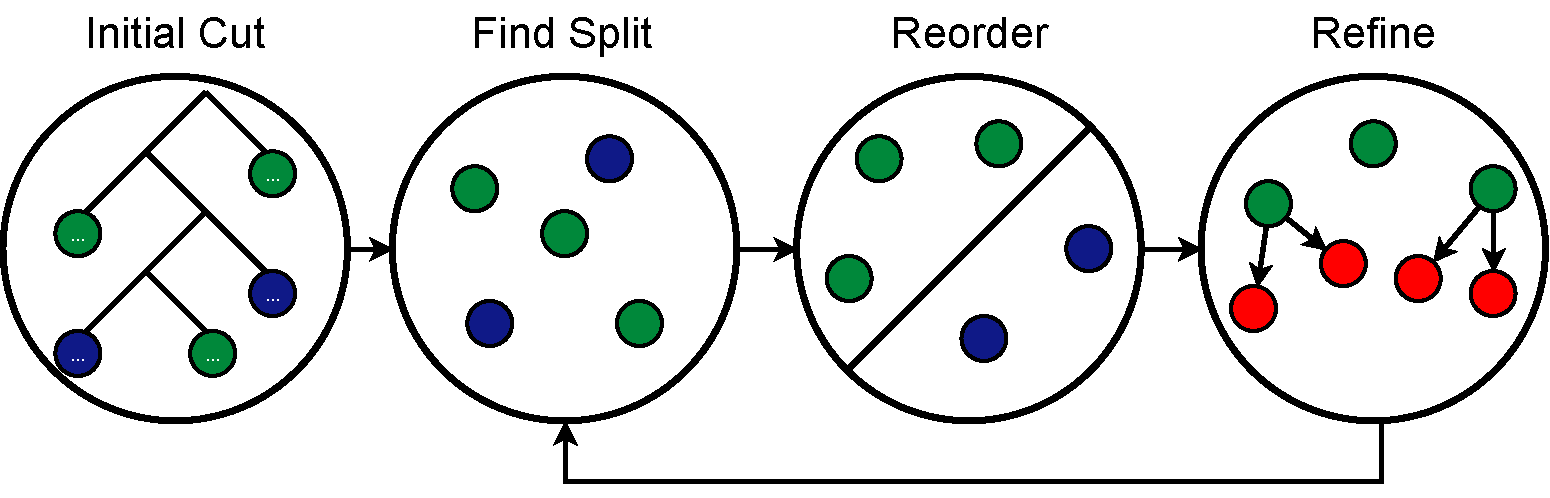
\includegraphics[width=400pt]{images/phr_algorithm.pdf}
    \caption{Illustration of the progressive hierarchical refinement algorithm.}
    \label{fig:phr}
\end{figure}
This section further explains the algorithm used to construct bounding volume hierarchies. Bounding volume hierarchies are constructed using progressive hierarchical refinement (PHR) as proposed by Hendrich et al.\cite{hendrich_parallel_2017}. As previously established, applying full sweep SAH to all scene primitives is magnitudes too slow. PHR tackles this problem by first constructing an auxiliary BVH, which then serves as a hierarchy to find much smaller sets of nodes on which full sweep SAH can be applied fairly inexpensively. The two resulting cuts are then refined, meaning that some nodes within those cuts are replaced by their children, if their bounding box surface area is above a certain threshold. Afterwards, the algorithm is applied recursively to the refined cuts until the full BVH is constructed. An illustration of that process can be seen in figure \ref{fig:phr}.

\subsection{Auxiliary Bounding Volume Hierarchy}
\label{aux}
As the auxiliary BVH is only needed as a description of the scene's hierarchy, construction speed is the main priority. Multiple fast builders have been tested in the original paper\cite{hendrich_parallel_2017}, but linear bounding volume hierarchies (\acrshort{lbvh}) turned out to be the best choice. LBVH was first proposed by Lauterbach et al.\cite{lauterbach09lbvh} as a top-down algorithm that assigns Morton codes to all primitives and then builds the tree as a binary radix tree. The algorithm itself has since been improved multiple times\cite{karras12lbvh,apetrei14lbvh,chitalu20lbvh} making it one of the fastest approaches to date\cite{meister21survey}. However, these approaches exploit the massive parallelism GPUs can provide by building the BVH in a bottom up fashion, which makes less sense on the limited amount of cores CPUs provide. Consequently, the approach used here is closer to the top-down algorithm proposed by Lauterbach et al.\cite{lauterbach09lbvh} with a few adjustments. 
\begin{figure}[H]
    \centering
    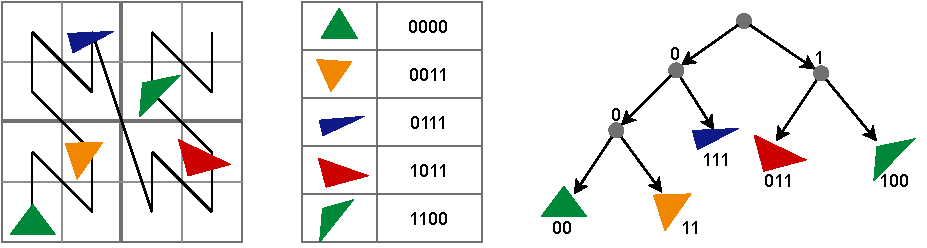
\includegraphics[width=400pt]{images/morton_curve.pdf}
    \caption{Left shows 2D Morton curve using 2 bits per dimension. The table in the center shows the corresponding Morton codes and the right shows the resulting tree structure, equivalent to a binary radix tree.}
    \label{fig:morton}
\end{figure}
Construction of the auxiliary BVH starts off by sorting all primitives along a Morton curve\cite{morton66curve}. This space filling curve subdivides the scene space into a uniform grid, resulting in Morton codes of fixed length (figure \ref{fig:morton}). Computation of Morton codes is done fairly efficiently by interleaving successive bits of the primitives' quantized bounding box centroids.

Morton codes are assigned in parallel by processing $[n/t]$ primitives per thread, with $n$ being the number of scene primitives and $t$ being the number of threads. Afterwards, the primitives are sorted according to their Morton code using a parallel bucket sort implementation. In each thread, $k=2^{12}$ empty buckets are created and filled with $[n/t]$ primitives. By using individual buckets for each thread, no further synchronization necessary for the bucketing. However, an atomic counter is used to keep track of the total number of primitives in each bucket across all threads, which is then used to find the intervals in the original array each bucket occupies. After bucketing is finished, all non-empty buckets with the same index are merged and directly written to the mentioned interval in the input array, before being sorted in place using Go's built-in sort function. This step is also done in parallel by utilizing the worker pattern to send buckets with the same index to each thread until all buckets have been processed.

The corresponding BVH can be constructed by recursively splitting the set of primitives at the highest bit within the current interval. This is done using a Go channel and entries representing a node in the finished tree. Each thread fetches such a node and finds the split in the corresponding array by applying linear search. If the node does not become a leaf, the resulting cuts are sent to the channel to be processed by idle threads.

Finally, the bounding boxes of the tree are updated in parallel by starting at the tree's leaves and traversing towards the root. Whenever a thread visits a node, the bounding box is updated using the child or primitive bounding boxes. Then the parents atomic counter is incremented and if all children are set, the thread also processes the parent. Otherwise, the thread fetches an unprocessed leaf from a queue. The same procedure is executed when refitting the LBVH on scene changes. 
\subsection{Algorithm}
\label{phr_algorithm}
The main progressive hierarchical refinement algorithm starts by identifying a set of nodes that separate root and leaves of the auxiliary LBVH. Nodes are selected in parallel using a priority queue. A thread pops an entry from that queue and compares its bounding volume surface area to a given threshold. If the surface area is below that threshold or the cut has reached its maximum size, the node is added to the initial cut. Otherwise, its children are inserted into the priority queue to be processed by another thread. The resulting cut is several magnitudes below the full primitive count and can be processed fairly inexpensively using full sweep SAH.

Cuts are split by evaluating an adapted version of the surface area heuristic for all three axis and choosing the split with the lowest cost. The cut becomes a leaf, if the cost of not splitting at all is the lowest. Each axis is evaluated by sorting nodes along given axis according to their bounding box centroid. The SAH cost for a split at the index $i$ in the sorted set is given as 
\[C(i)=S_L(i)n_L(i)+S_R(i)n_R(i)\]
where $S_L(i)$ and $S_R(i)$ are the bounding boxes surface areas of the left and right subsets and $n_L(i)$ and $n_R(i)$ are the number of nodes in the corresponding subtrees. Note that this expression is very similar to the SAH cost presented in section \ref{acceleration_structure_basics}. However, instead of using the number of primitives in the left and right cuts, the number of nodes is used. According to Hendrich et al.\cite{hendrich_parallel_2017}, this improves the performance by a few percent, as the number of nodes better reflects the complexity of the given subtree.

The SAH evaluation algorithm first computes all right costs $S_R(i)n_R(i)$ by incrementally extending the split bounding box and storing the partial costs, which is more efficient than computing the full bounding box at each step. The full cost is then calculated in the same fashion, extending the bounding box from the left to solve $S_L(i)n_L(i)$. 

Splitting the cut reduces the number of nodes in each new cut and doing so multiple times would lead to a cut size of one. To keep cuts at a larger size for longer and to better utilize the hierarchical information the auxiliary BVH can provide, cuts are refined after splitting. Keeping cuts at a constant size, as proposed by Hunt et al.\cite{hunt07lazybuild}, would become rather expensive towards the bottom of the tree due to the growing number of cuts. As a solution, Hendrich et al.\cite{hendrich_parallel_2017} proposed an adaptive refinement approach based on the current depth in the tree. This approach makes cuts shrink towards the bottom of the tree, which balances the computational cost between different levels of the tree. The BVH quality is not worsened significantly by doing so, as the impact of SAH gets lower further down the tree. 

Refinement works by comparing node bounding box surface areas to an adaptive threshold. Nodes with a surface area below this threshold are kept within the cut. Otherwise, the node is replaced by its children. This adaptive threshold is given as 
\[t_d = S /{2^{\alpha d + \delta}}\]
with $S$ being the surface are of the scene bounding box and $d$ the current depth in the tree. The parameter $\alpha$ describes how quickly cuts shrink towards the bottom and $\delta$ determines the size of the initial cut for $d=0$. The setting of these parameters determines the build-trace trade-off of the algorithm and is elaborated further in section \nameref{parameters}.

Construction of the BVH uses a similar setup as previously mentioned for the LBVH generation. A thread pool of $t$ threads pops entries from a channel, consisting of a cut and parent node index. The cut is split using the described method, the resulting cuts are refined and then fed back into the channel if the node did not become a leaf. Additionally, a higher branching factor can be specified to build a multi-BVH\cite{wald08multibvh}. In that case, a thread keeps splitting the biggest resulting cut until enough children have been generated or no more splits exist. The effect of multi-BVHs on the rendering performance is evaluated in section \ref{multi_bvh}.

\begin{figure}[H]
    \centering
    \subcaptionbox{Render}{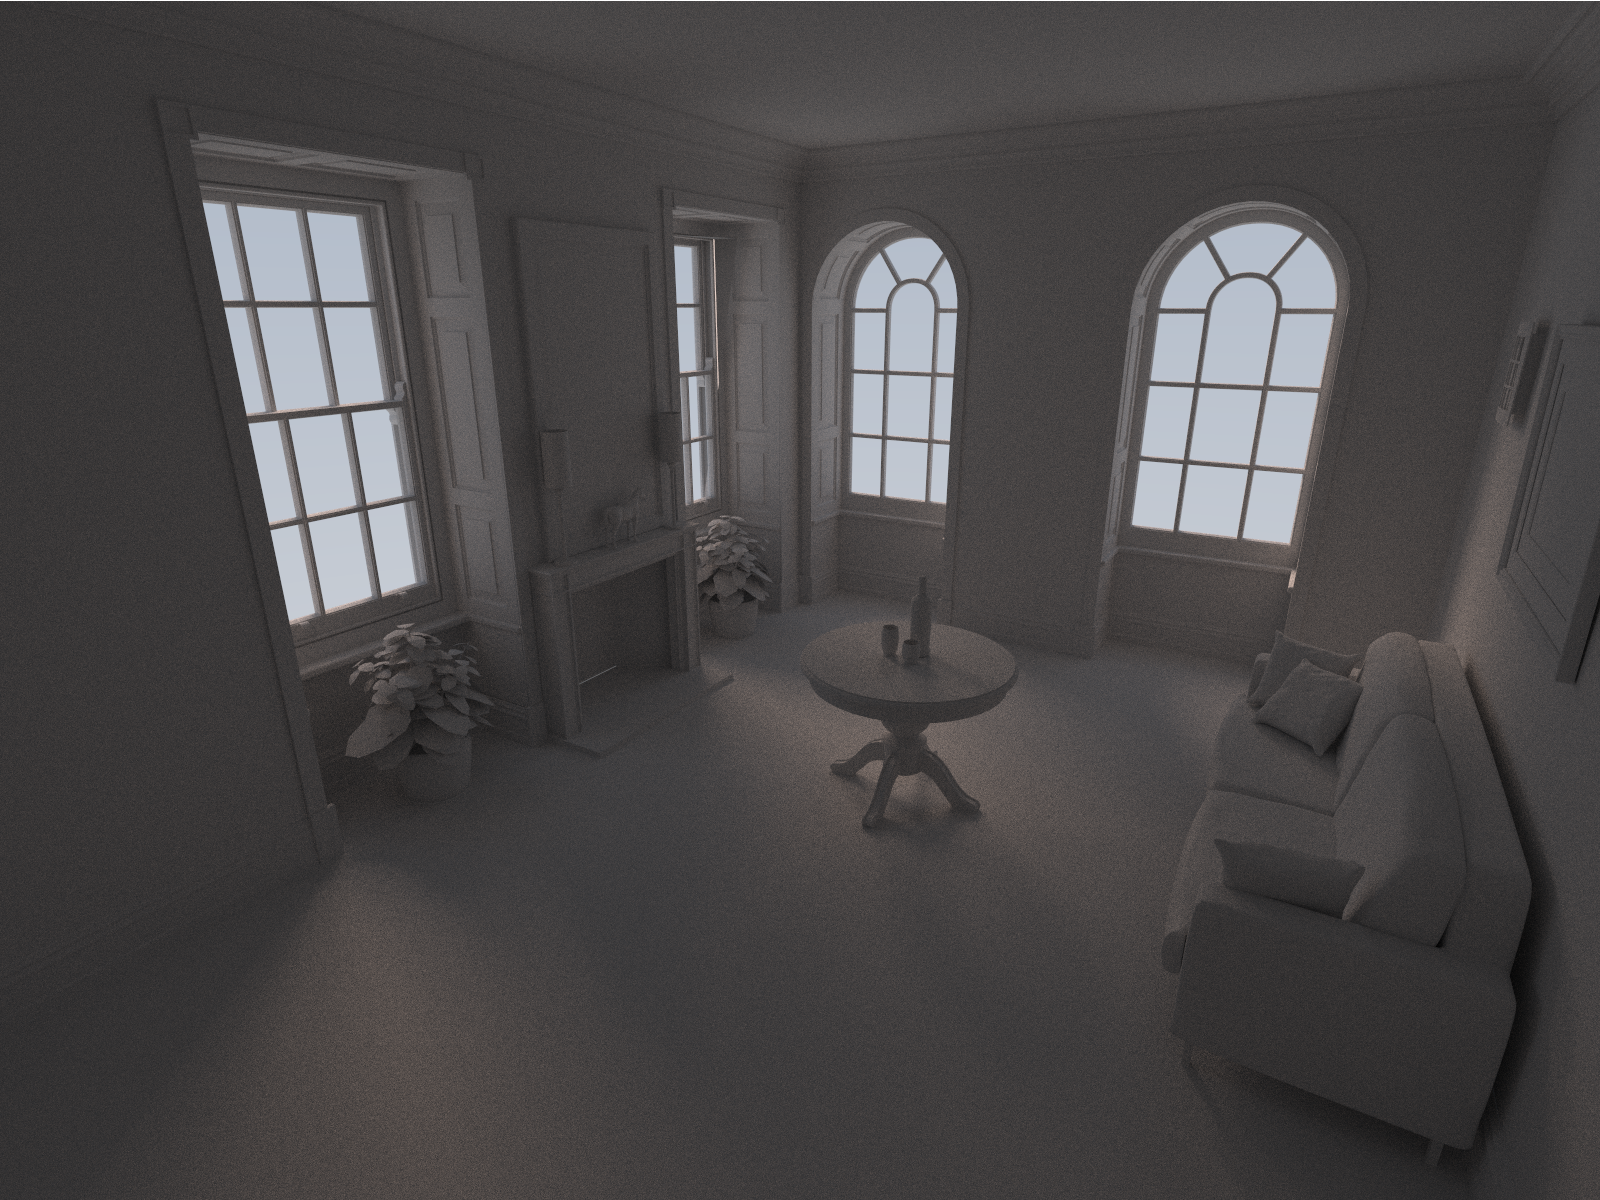
\includegraphics[width=0.3\textwidth]{images/fireplace_render.png}}
    \hfill
    \subcaptionbox{LBVH}{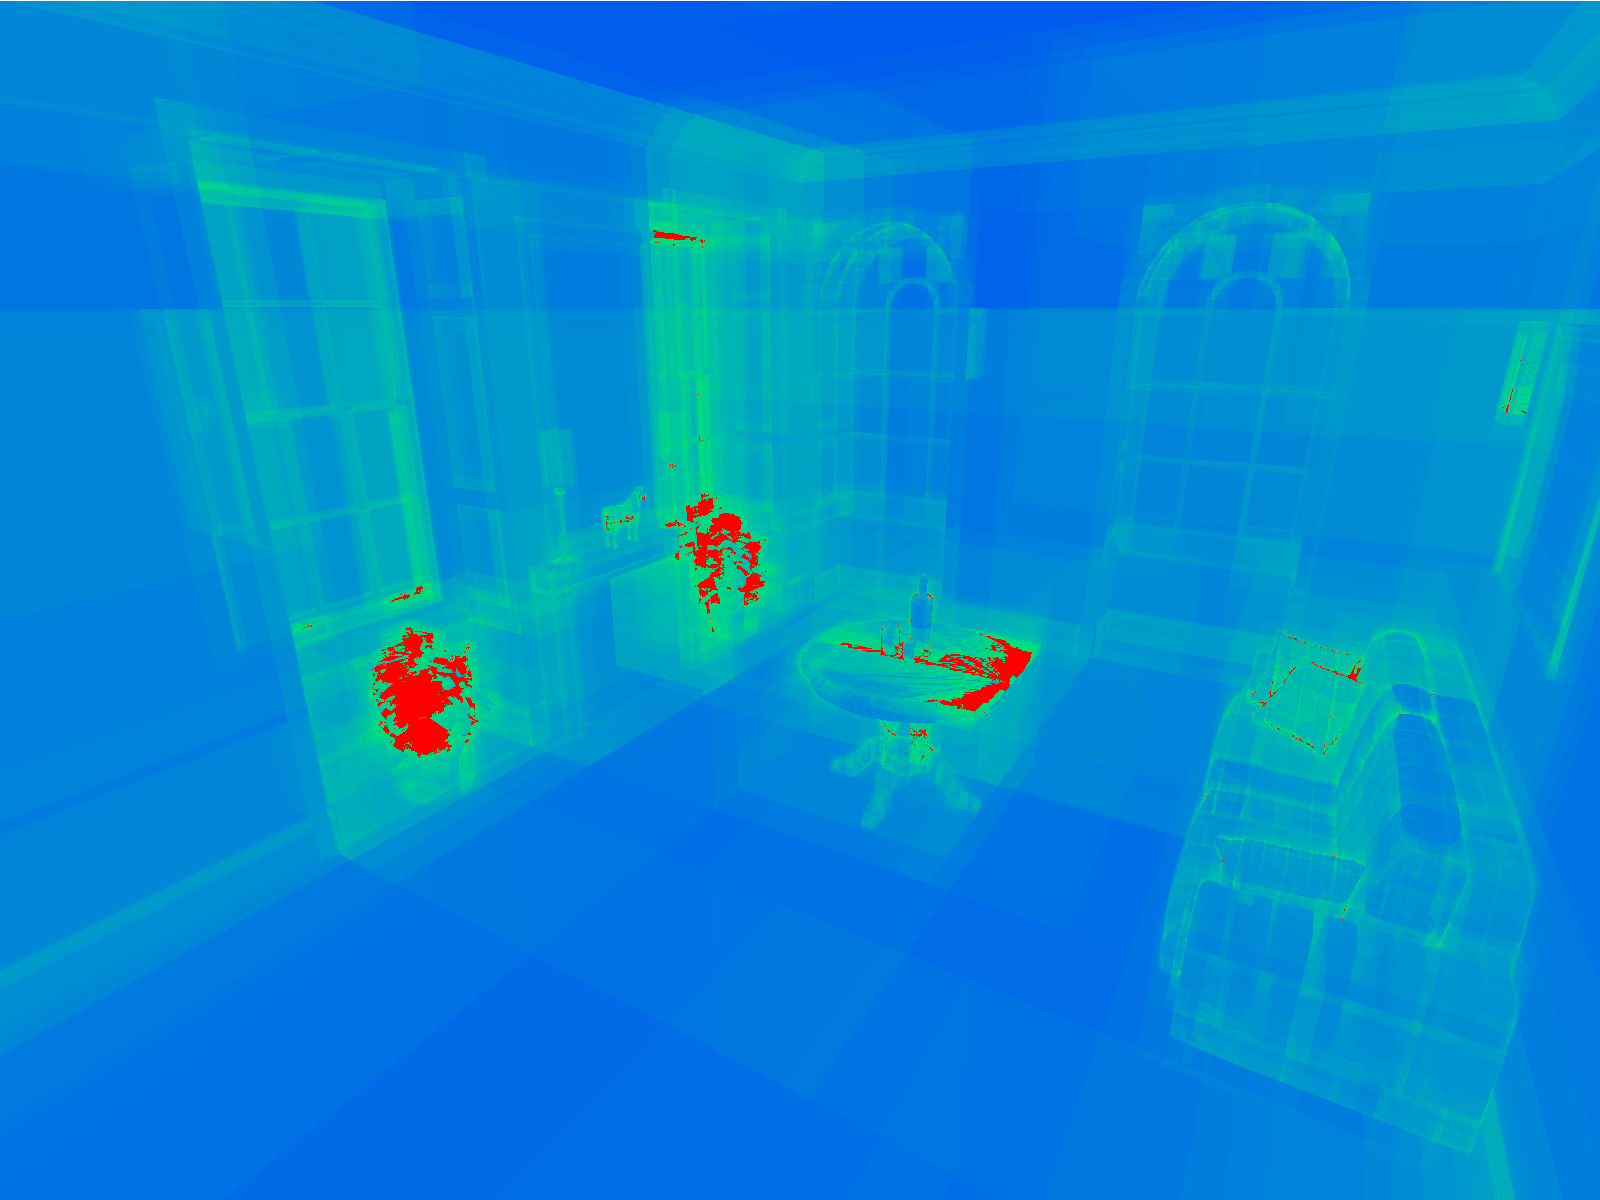
\includegraphics[width=0.3\textwidth]{images/fireplace_lbvh.png}}
    \hfill
    \subcaptionbox{PHR-HQ}{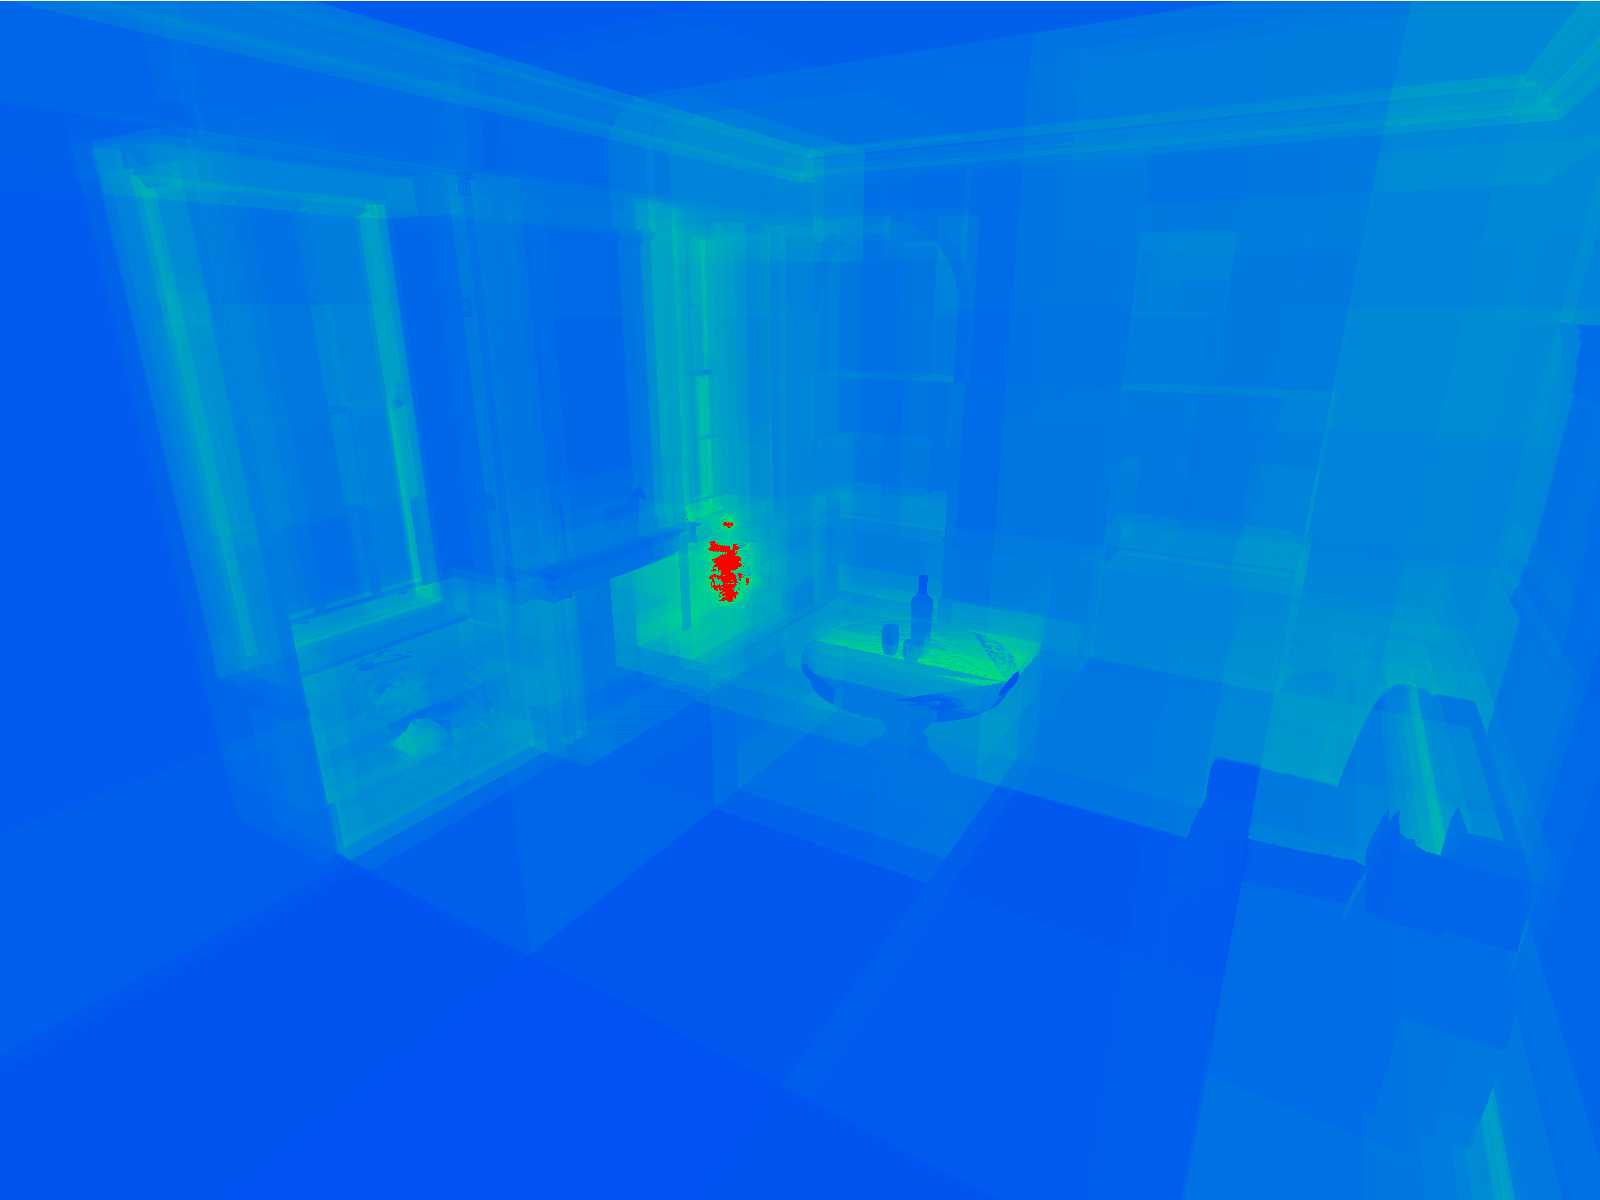
\includegraphics[width=0.3\textwidth]{images/fireplace_phr.png}}
    \caption{Visualization of the number of traversal steps for primary rays using LBVH and PHR (red color corresponds to 100 traversal steps per ray).}
    \label{fig:noise}
\end{figure}
\subsection{Integration into Interactive Path Tracing}
\label{phr_in_interactive}
An approach for integrating progressive hierarchical refinement into interactive applications was mentioned in the original paper\cite{hendrich_parallel_2017}, but its validation remained an open topic. The idea was to only build the auxiliary BVH once in the beginning and then refit it very efficiently between frames. Refitting is done by updating bounding boxes of all BVH nodes. The hierarchy of the structure stays unchanged during this procedure. As described in the end of section \ref{aux}, this is done using a parallel recursive procedure that traverses the tree in a bottom-up fashion and merges child bounding boxes using an atomic counter for synchronization. Doing so is fairly efficient in comparison to a full BVH rebuild, however, refitting generally leads to some extend of BVH quality loss, especially for significant scene changes. Applying PHR to the refitted tree counteracts this loss by building a new BVH.
\cleardoublepage
\section{Hyperparameters}
\label{parameters}
This section proposes an equation to evaluate the build-trace trade-off of the PHR algorithm. Two possible solutions for the optimization problem are them presented in the form of grid search and Bayesian optimization. As established in the previous section, PHR depends on the parameters $\alpha$ and $\delta$ describing initial cut size and shrink rate. These parameters can be set to adjust the trade-off between build time and trace performance. However, the optimal parameters can differ between scenes and view points, especially when dealing with dynamic scenes and refitted auxiliary trees.
% TODO: Add figure that shows different optimal parameters and prove thesis
Frame size also plays a role as higher resolutions profit more from well optimized bounding volume hierarchies while the hit taken by the extended build time is not as significant given the overall higher computational effort. 
\subsection{Evaluation}
\label{evaluation}
Ultimately, the overall frame time including BVH build time and render duration needs to be minimized to unlock the full potential of progressive hierarchical refinement. Stopping the actual execution times is neither efficient nor reliable enough, so an efficient metric that makes the trade-off quantifiable is needed. 

A number of metrics have been proposed to estimate the quality of a given bounding volume hierarchy. A well known cost model based on the surface area heuristic, taken from \cite{meister21survey}, is given by the recurrence equation 
\[
c(N) =  
    \begin{cases}
        c_T + \sum_{N_c}P(N_c|N)c(N_c) &\quad\text{if }N\text{ is interior node,}\\
        c_I|N|&\quad\text{otherwise}\\
    \end{cases}
\]
where $C(N)$ is the cost of the subtree with root $N$, $N_c$ is a child of node $N$, $P(N_c|N)$ is the conditional probability of traversing node $N_c$ when $N$ is hit and $|N|$ is the number of primitives in the subtree with root $N$. 

Constants $c_T$ and $c_I$ express the average cost of a traversal step and ray-primitive intersection, respectively. Utilizing the micro-benchmarking capabilities of Go revealed that a triangle intersection takes approximately 7 nanoseconds on average, while a traversal step takes around 12 nanoseconds. Consequently, these constants are set to $c_T = 2$ and $c_I = 1$, roughly representing the ratios between those values. 
The conditional probabilities of traversing a node are expressed using the surface area heuristic\cite{goldsmith_automatic_1987,macdonald_heuristics_1990}
\[
P(N_c|N)^{SAH} = \frac{SA(N_c)}{SA(N)}
\]
where $SA(N)$ and $SA(N_c)$  are the bounding box surface areas of nodes $N$ and $N_c$, respectively. 

Evaluating the build complexity of PHR given a set of parameters and an arbitrary scene is not as trivial, as there is no clear correlation between the parameter values and associated build times.  
\begin{figure}
    \centering
    \subcaptionbox{Build Time}{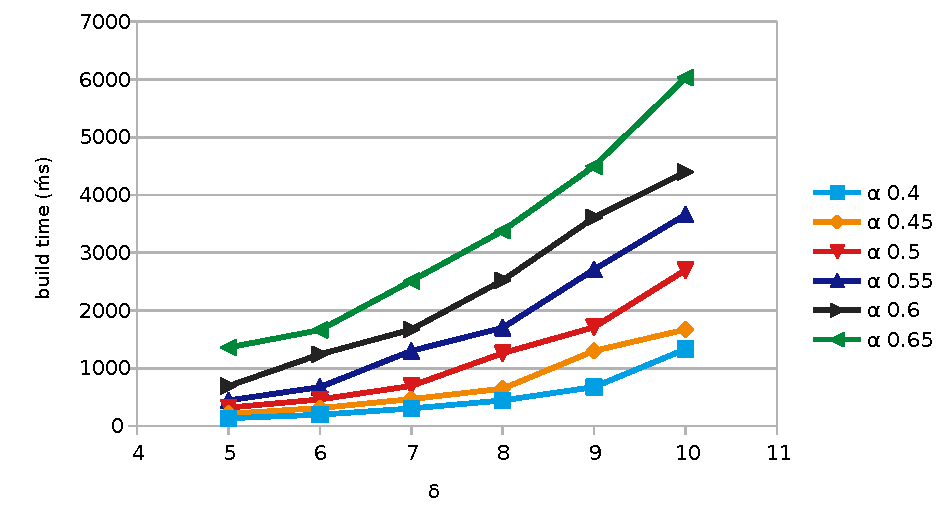
\includegraphics[width=0.45\textwidth]{images/build_time.pdf}}
    \hfill
    \subcaptionbox{Build Cost}{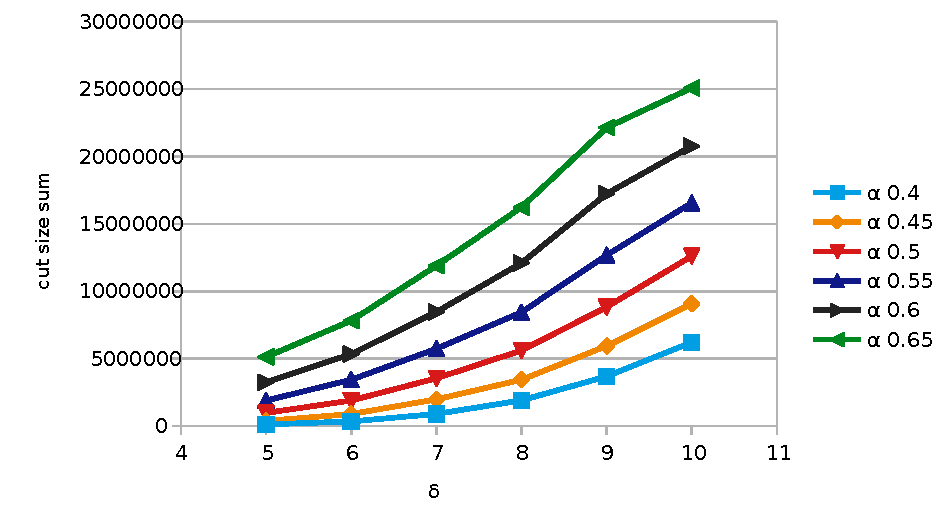
\includegraphics[width=0.45\textwidth]{images/build_cost.pdf}}
    \caption{Both the build time and corresponding build cost for the San Miguel scene. This corresponds to a correlation of 0.994.}
    \label{fig:build_cost}
\end{figure}
For scenes with medium to high complexity, the tree size of the resulting BVH could be used as a metric with an average correlation coefficient of around 0.98 between tree size and build time. This correlation does not hold true for simpler scenes though, as trees stop growing once no favorable splits can be found anymore.
A better metric is the total sum of all cut sizes, as seen in figure \ref{fig:build_cost}, which can be obtained through a minimal adjustment of the progressive hierarchical refinement algorithm. The surface area heuristic evaluation is the most expensive part of PHR and thus the total number of evaluated nodes directly correlates with the execution duration. Using an atomic counter, the performance penalty is very marginally to non existing. Furthermore, an alternative implementation can be used for the optimization process. The correlation between this number and the BVH construction time averages to 0.99 across all tested scenes.

Let the build cost $b$ be defined as
\[
    b(\alpha, \delta) = \sum_{cut\in PHR'(\alpha, \delta)}|cut|
\]
where $b(\alpha, \delta)$ is cost of a PHR execution given the parameters $\alpha$ and $\delta$, $PHR'(\alpha, \delta)$ is a execution of the progressive hierarchical refinement algorithm resulting in a set of all cuts processed and $|cut|$ is the length of given cut.

I propose an equation to evaluate the combined cost of a frame rendered using the PHR algorithm, which also factors in the build-trace trade-off. Given a pair of parameters $\alpha$ and $\delta$, this cost is defines as
\[
    e(\alpha,\delta) = ||b(\alpha,\omega)|| + \omega^2 ||c(PHR(\alpha,\omega))||
\]
with $||b(\alpha,\delta)||$ being the normalized build cost and $||c(PHR(\alpha,\omega))||$ the normalized SAH cost of the resulting BVH. The coefficient $\omega$ functions as a weight determining to what extend trace performance should be favored over build duration. For $\omega=1$, both trace and build performance are weighed equally, $\omega>1$ favors higher trace speed and $\omega<1$ encourages faster build times. These trade-off depends on scene complexity and frame size, so $\omega$ is defined as:
\[
    \omega = (\frac{|prim|}{\omega_p})^2 * (\frac{w*h}{\omega_r})
\]
where $|prim|$ is the total number of primitives in the scene and $w$ and $h$ are width and height of the rendered frame, respectively. $\omega_p$ and $\omega_r$ are constants depending on the performance of the used path tracer and the targeted frame rate, so they stay constant across all scenes. $\omega_p$ expresses a number of primitives and $\omega_r$ a frame size at which the trade-off should be equal, i.e. $\omega=1$. Once those numbers are exceeded, BVH quality is favored increasingly. 

Combining the equation with the previously mentioned metrics and given a search space over the parameters $\alpha$ and $\delta$ (e.g. $\alpha\in A=[0.4,0.6], \delta\in D=[5,10]$) leads to the expression:
\[
    e(\alpha,\delta) =
        \frac{b(\alpha, \delta)}
        {\max_{\alpha\in A,\delta\in D}b(\alpha, \delta)}
        + \omega^2
        \frac{c(PHR(\alpha, \delta))}
        {\max_{\alpha\in A,\delta\in D}c(PHR(\alpha, \delta))}
\]
where $PHR(\alpha,\delta)$ is a execution of the PHR algorithm using the parameters $\alpha$ and $\delta$ resulting in the root node of a bounding volume hierarchy.
\clearpage
\subsection{Grid Search}
The brute force approach grid search is the obvious first choice to solve this optimization problem. A number of possible values is chosen for each parameter (e.g. $\alpha\in\{0.45,0.5,0.55\}$ $\delta\in\{5,6,7,8\}$) and all possible combinations are tested and evaluated. By postponing the evaluation of $e(\alpha,\delta)$ until all individual cost evaluations $b(\alpha, \delta)$ and $c(PRH(\alpha,\delta))$ are available makes their maxima directly accessible, which is another advantage of grid search. 

Usually, grid search would be too costly for such a time critical task. In this case however, only two parameters need to be optimized and the search space is relatively small making grid search a potentially viable approach. 

\subsection{Bayesian Optimization}
A more efficient approach compared to grid search is Bayesian optimization\cite{pelikan99boa}, which explores the search space by taking previous observations into account. This is done by placing a prior probability distribution over the objective function $e(\alpha,\delta)$. First, parameters $\alpha$ and $\delta$ are chosen by random in the given search space. Following their evaluation, the prior is updated to form a posterior distribution. Based on this posterior distribution, an acquisition function is constructed to select the next point worth exploring. 

In particular, the Bayesian optimizer\cite{ou19bo} utilizes a Gaussian process to define the prior/posterior distribution, and expected improvement is used as exploration strategy.

One issue compared to the aforementioned grid search approach is, that the maximum BVH and build costs are not directly available when evaluating $e(\alpha,\delta)$. This is solved by running PHR once with the lowest possible parameters in the search space to obtain the maximum BVH cost and once with the highest possible parameters to obtain the maximum build cost. These numbers correspond to the respective maxima very reliably and there evaluations can also be factored into the prior probability distribution.
\cleardoublepage
\section{Results}
\label{results}
Both the BVH builder and path tracer were implemented in Go and only utilize the CPU. Code is optimized moderately without exploiting any SIMD instructions. A series of tests was conducted to compare the build times, ray tracing performance and resulting time per frame rendered between different hyperparameter configurations. LBVH was used as reference, PHR-Fast and PHR-HQ used the parameters proposed by Hendrich et al.\cite{hendrich_parallel_2017}, namely $\alpha=0.5, \delta=6$ and $\alpha=0.55, \delta=9$, respectively. PHR-Grid uses parameters based on the proposed grid search approach over the search space $\alpha\in\{0.4,0.45,0.5.0.55\}, \delta\in\{6,7,8,9\}$ and PHR-BO uses parameters resulting from a Bayesian optimization over the equivalent interval $\alpha\in[0.4,0.55], \delta\in[6,9]$. The Bayesian optimization itself is executed utilizing the bo framework\cite{ou19bo} and is based on a Gaussian process and expected improvement as exploration strategy. 

To make results more reliable, all numbers were averaged over ten executions using the bench framework\cite{ou20bench}. Furthermore, the CPU, an AMD Ryzen 2600 eight core processor with 3.4 GHz, was locked to 90 percent capacity to prevent irregularities due to overheating or other high performance fluctuations. Note that the deviation percentages are left out for clarity in the tables presented in this thesis, but the full results are available in the attached files. 

Render times are also averaged over three representative views for each scene. To keep times in an interactive window, only the relatively small resolutions 256x256 and 512x512 were tested with one sample per pixel. 
\subsection{Multi-Bounding Volume Hierarchies}
\label{multi_bvh}
As mentioned in section \ref{phr_algorithm}, the PHR algorithm allows the construction of bounding volume hierarchies with higher branching factors, which is especially useful for SIMD path tracers. Even though the evaluated path tracer does not utilize any SIMD instructions, I compared the build and trace performance of different multi-BVHs. As expected, the performance difference between branching factors was insignificant in most cases. 4-ary BVHs had slightly faster trace times, while 16-ary BVH construction was slightly slower. The following tests were all performed on 2-ary BVHs. 
\subsection{Frame Performance}
The main part of the experiment was about comparing the resulting frame times of all configurations. Table \ref{tab:frametime} shows build time, SAH cost, average render time over the compared view points and the resulting frame times. Note that the PHR build times do not include construction of the auxiliary bounding volume hierarchy, as those would be reused over several frames. 

First of all, the numbers clearly show the impact different PHR parameters can have on the build and trace time of the algorithm. PHR-Fast was indeed fairly fast, but the achieved trace speed is even below the baseline, LBVH, in some cases. PHR-HQ had the fastest trace speed in most cases, but the high build duration often leads to higher frame times. A noticeable difference can be seen between the different scene types. PHR performed comparably worse in single object scenes like Bunny, Dragon and Happy Buddha, often not exceeding the render performance of LBVH by much. Sibenik's and Sponza's render times on the other hand, were improved more significantly by applying PHR. Finally, PHR-Grid and PHR-BO were able to improve frame times significantly in a number of cases. However, Bayesian optimization delivered rather inconsistent results and no approach was able to find the optimal parameters in every case. This is probably a result of overfitting the evaluation function and their parameters to certain scenes. Nonetheless, both PHR-Grid and PHR-BO are able to improve frame times compared to PHR-Fast and PHR-HQ. Figure \ref{fig:difference} shows the average relative performance compared to LBVH in percent. While PHR-Fast only improves frame times by 33\% on average, both optimization approaches surpass an average improvement of 50\%.
\begin{figure} [H]
    \centering
    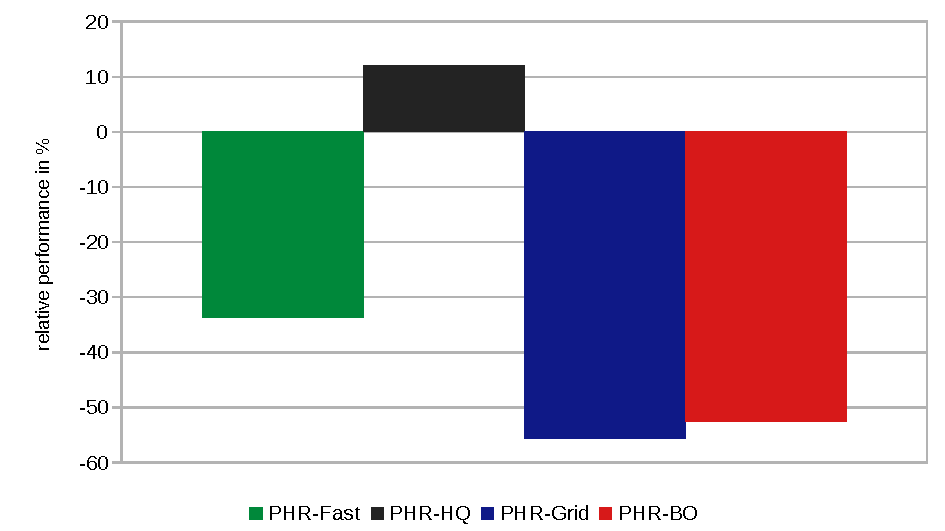
\includegraphics[width=300pt]{images/performance_difference.pdf}
    \caption{Relative difference to LBVH in percent.}
    \label{fig:difference}
\end{figure}
\subsection{Optimization Performance}
Figure \ref{fig:optimization} shows optimization times divided through average frame time, or in other words, how many frames could potentially be rendered instead of executing the optimization. Considering that the average performance increase of both methods amounted around 50\%, i.e. can potentially half the rendering time, optimizations start to become viable at half a frames duration and below. So even though the search space used in grid search is relatively low, the achieved times never reached what would be feasible in interactive applications. Bayesian optimization performed considerably better, but only reached competitive times in a few cases. Note that reaching this time does not equal a performance increase but just a hypothetical chance that frame times are increased. 

This shows that the presented optimization approaches still lack in performance and are not yet viable. PHR needs to be executed to evaluate the cost function, which is especially costly for parameters that result in high build times. This could be improved by limiting the search spacer further or making it dynamic and related to the scene's complexity. An interrupt after a maximum execution time might also be a solution. Bayesian optimization uses a costly run with maxed out parameters to determine the maximum build cost. This could be solved by reusing max values from previous optimizations. This topic is discussed further in section \ref{discussion_execute}.
\begin{figure}[H]
    \centering
    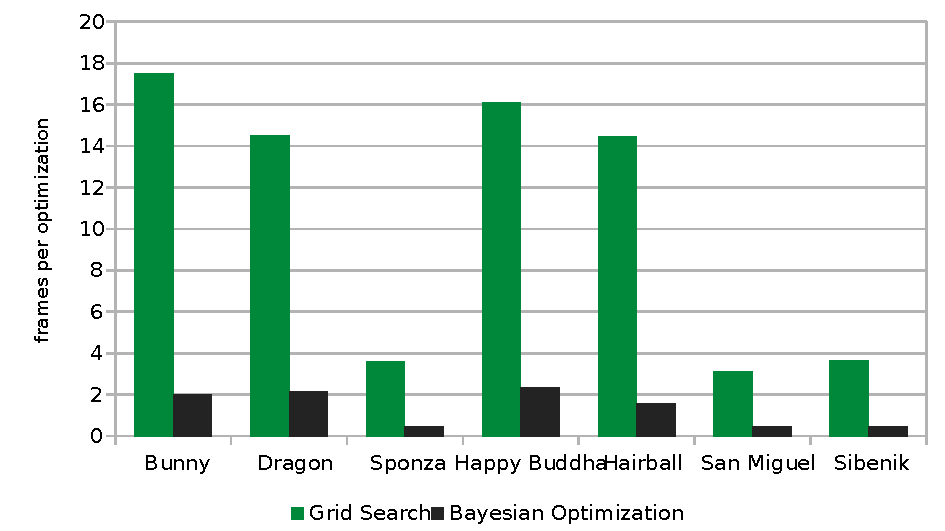
\includegraphics[width=300pt]{images/frame_per_optimization.pdf}
    \caption{Number of potential frames during optimization.}
    \label{fig:optimization}
\end{figure}
\clearpage
\begin{table}
\caption{Performance comparison of a representative selection of tested configuration at 256x256 resolution.}
\label{tab:frametime}
\centering
\begin{tabular}{ | c | m{3.5em} | m{3.5em} | m{3.5em} | m{3.5em} | m{3.5em} |  m{3.5em}|}
\hline
& build time (ms) & render time (ms) & frame time ms & build time (ms) & render time (ms) & frame time ms\\
\hline
& \multicolumn{1}{|m{4.5em}}{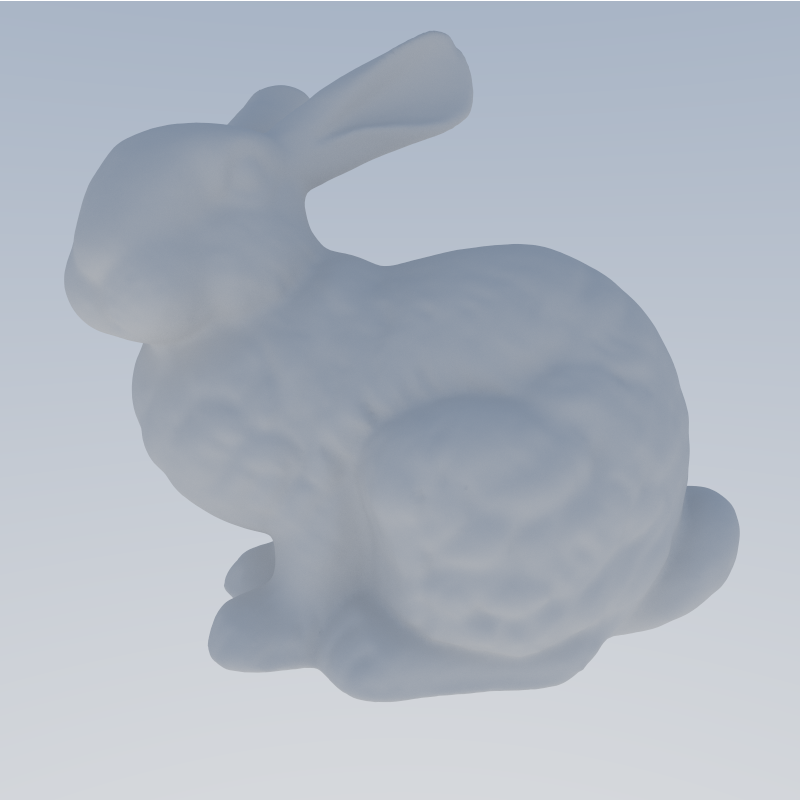
\includegraphics[width=60pt]{images/bunny.png}} &     \multicolumn{2}{m{4em}|}{Bunny \#triangles 144k} 
& \multicolumn{1}{|m{4.5em}}{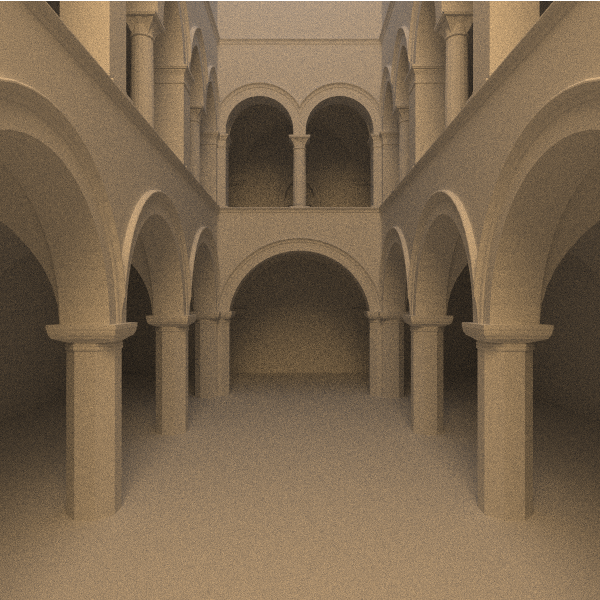
\includegraphics[width=60pt]{images/sponza.png}} & \multicolumn{2}{m{4em}|}{Sponza \#triangles 66k}\\
\hline
LBVH & 152.0 & 21.9 & 173.9            & 70.4 & 227.0 & 297.5 \\
PHR-Fast & 70.5 & 20.1 & 90.6          & 27.6 & 184 & 211.6 \\
PHR-HQ & 273.0 & 20.7 & 293.7          &  94.7 & 182 & 276.7\\
\hline
PHR-Grid & 14.4 & 20.8 & 35.2        &  17.2 & 207 & 224.2\\
PHR-BO & 14.2 & 20.7 & 34.97         &  21.7 & 200 & 221.7\\
\hline
& \multicolumn{1}{|m{4.5em}}{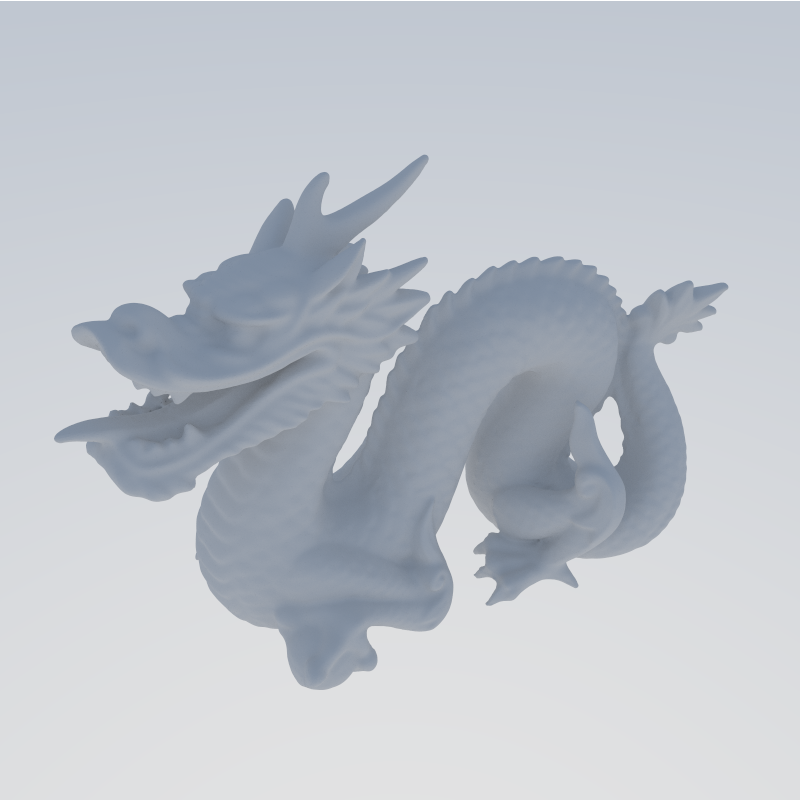
\includegraphics[width=60pt]{images/dragon.png}} &     \multicolumn{2}{m{4em}|}{Dragon \#triangles 817k}

& \multicolumn{1}{|m{4.5em}}{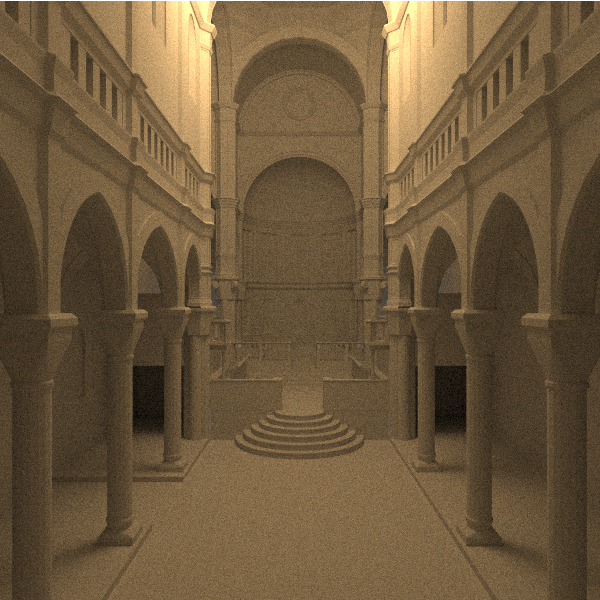
\includegraphics[width=60pt]{images/sibenik.png}} & \multicolumn{2}{m{4em}|}{Sibenik \#triangles 75k}\\

\hline
LBVH & 900.0 & 28.1 & 928.2              &  72.1 & 226.1 & 298.1\\
PHR-Fast & 150.0 & 32.5 & 182.5            &  32.5 & 205 & 237.5\\
PHR-HQ & 1090.0 & 29.0 & 1119.0              &  98.4 & 187  &285.4\\
\hline
PHR-Grid & 31.7 & 63.5 & 95.2            & 19.1 & 236 & 255.1  \\
PHR-BO & 30.8 & 66.1 & 96.9              & 28.1 & 220 & 248.1 \\
\hline
& \multicolumn{1}{|m{4.5em}}{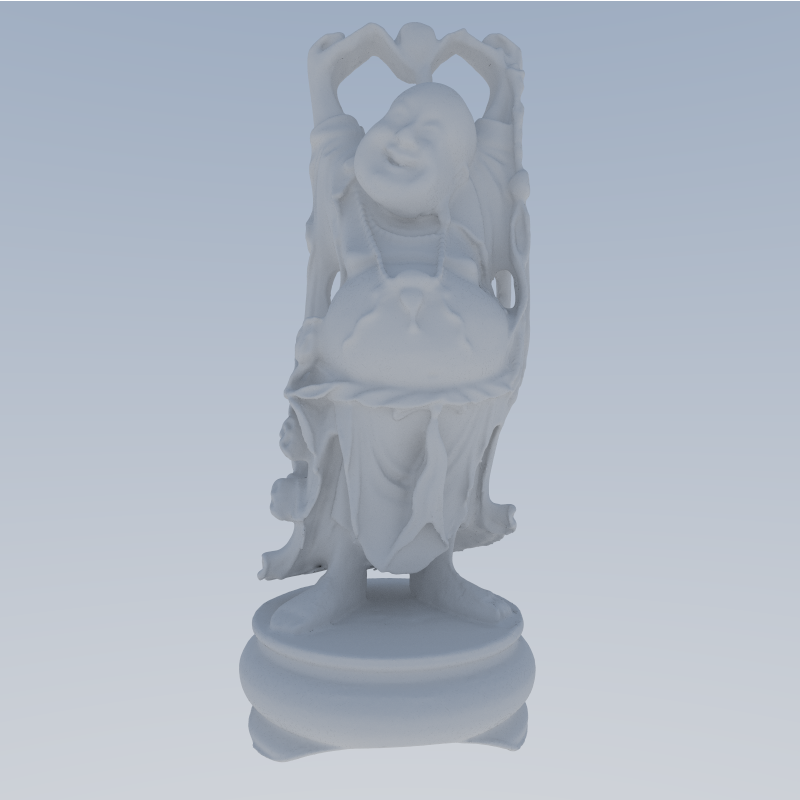
\includegraphics[width=60pt]{images/buddha.png}} & \multicolumn{2}{m{4em}|}{Happy Buddha \#triangles 1087k}

& \multicolumn{1}{|m{4.5em}}{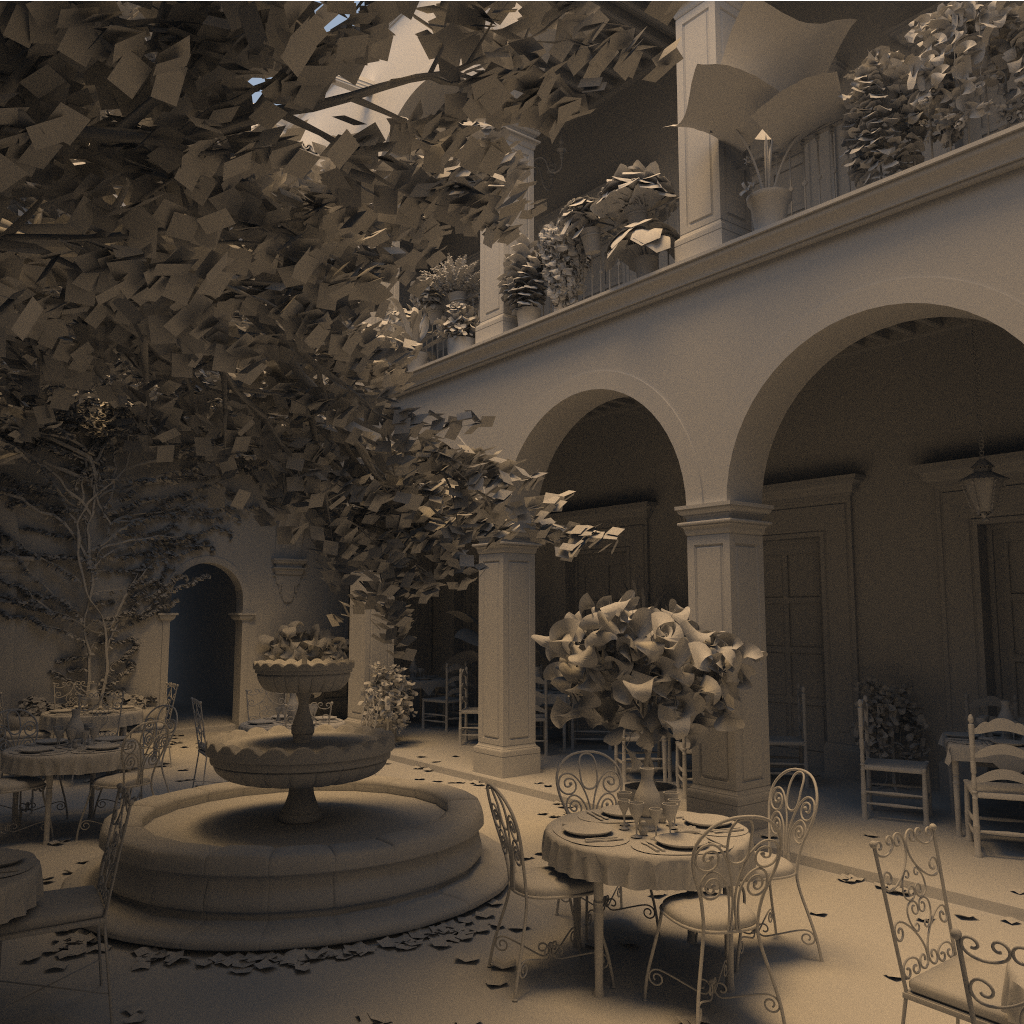
\includegraphics[width=60pt]{images/san_miguel.png}} &     \multicolumn{2}{m{4.5em}|}{San Miguel \#triangles 5617k}\\


\hline
LBVH & 1080 & 25 & 1105                    & 6010.0 & 816.0 & 6826.6 \\                   
PHR-Fast & 190 & 27.6 & 217.6                   & 432.0 & 7830.0 & 8262.0 \\
PHR-HQ & 1250 & 23.7 & 1273.7                     & 2600.0 & 812.3 & 3412.3 \\
\hline
PHR-Grid & 40.5 & 57.5 &98                   & 1300.0 & 1856.6 & 3156.6  \\
PHR-BO & 42.1 &58 &100.1                     & 815.0 & 3203.3 & 4018.3 \\
\hline
\end{tabular}
\end{table}
\cleardoublepage
\section{Discussion}


\section{Conclusion}

\subsection{Further Work}
Path tracing is a very extensive topic and especially considering the task of writing a complete path tracer, there is a lot of work left open. Considering the path tracer, a missing but essential aspect is denoising. As discussed earlier, recently a lot of progress has been achieved in that field of research and integrating some of that into this project would be an interesting addition. Importance sampling is another technique that was not considered in this work, but might improve it a decent amount. 
Staying with the main focus of this thesis, replacing LBVH with another fast BVH builder could bring interesting results. The full sweep SAH at the core of PHR is still relatively expensive and might be replacable by the more efficient binning SAH for better performance, or extended by using other cost functions like ray distribution heuristic or occlusion heuristic. Finally, optimization of PHRs hyperparameters is not ideal yet and might be improved by either using other optimization procedures, or improving the evaluation function.
\cleardoublepage
\printglossaries
\cleardoublepage
\part*{Bibliography}
\addcontentsline{toc}{part}{Bibliography}
\nocite{*}
\bibliographystyle{apalike}
\bibliography{literatures/list}
\end{document}